\chapter{関数}\label{chapt_function}

%知るを知るとし, 知らざるを知らずとす。これ知るなり(孔子)。\hv

\section{関数のグラフ}

\underline{関数}\index{かんすう@関数} (function)
とは, 何か数を与えると, その数に応じて何か決まった数を返すような, 
対応関係のことである(定義)。例えば関数$y=x^2$は, 実数$x$を与えると, 
その2乗を$y$として返す。この場合, $x=3$を与えると, $y=3^2=9$を返す
\footnote{関数は, この例のように, 数式で表される
ことも多いが, 数式で表すことのできない関数もある。数を
与えるとそれに応じて決まった数を返す, という対応関係が
はっきりしていれば, 必ずしもその対応関係が数式で表されなくてもよいのだ。}。

関数を語るときの一般論の中では, 関数を$y=f(x)$と表すことが多い
(上の例では$f(x)$は$x^2$である)。別に$f$でなくても$a(x)$で
も$b(x)$でも何でもいいのだが, とりあえずfunctionの頭文字を
とって$f$をよく使う。

$x$に何かの値を与えると, $y=f(x)$から$y$の値が求められる。
このとき, 与えられる数(この場合は$x$)を\underline{独立変数} 
\index{どくりつへんすう@独立変数}
%(independent variable)
もしくは引数(ひきすう)\index{ひきすう@引数}といい, 求められる数(この場合は$y$)
を\underline{従属変数} \index{じゅうぞくへんすう@従属変数}
%(dependent variable)
という(定義)。

いろんな自然現象や社会現象は関数で表現され, 関数で予測される。
そのための数学, つまり関数を取り扱う数学を
「解析学\index{かいせきがく@解析学}」という。解析学の第一歩は, 
いろんな関数を適切にグラフに描くことである。

なお, この章では, 出てくる数は全て実数とする (複素数を扱う関数も存在するが, 
この章では考えない)。

さて, 最も単純な関数は「定数関数」\index{ていすうかんすう@定数関数}だ。
定数関数とは, 独立変数がどのような値であっても, 従属変数の値が
いつも同じ定数であるような関数である(定義)。
\begin{exmpl} 
\begin{eqnarray}y=1\label{eq:ex_constfunc1}\end{eqnarray}
は定数関数だ。式に$x$が入っていないから, $x$がどんな値を取ろうが無関係に, 
$y$の値は1。グラフは図\ref{fig:const}のように$x$軸に平行な直線になる。
(例おわり)
\begin{figure}[h]
    \centering
    \includegraphics[width=5cm]{const.eps}
    \caption{定数関数 $y=1$のグラフ。}\label{fig:const}
\end{figure}\end{exmpl}\mv
\begin{freqmiss}{\small\textgt{グラフに原点O, $x$軸の先の$x$, $y$軸の先の$y$等の記入を忘れる}
... グラフには, 原点(O), $x$軸(矢印と$x$), $y$軸(矢印と$y$)を必ず描き込むこと。}\end{freqmiss}

さて, 次に単純なのは, 中学校で習った
\begin{eqnarray}y=2x\label{eq:ex_propfunc2}\end{eqnarray}
のような関数だ。$y=2x$は, $x=0, 1, 2, \cdots$のときに, それぞれ
$y=0, 2, 4, \cdots$のような値をとる。グラフは図\ref{fig:proportion}の左側の
ように, 原点を通る, 右上がりの直線だ。一方, $y=-2x$のような関数のグラフは, 
図\ref{fig:proportion}の右側のように, 原点を通る, 右下がりの直線になる。
\begin{figure}[h]
    \centering
    \includegraphics[width=8.5cm]{proportion.eps}
    \caption{比例関係 $y=2x$と$y=-2x$のグラフ}\label{fig:proportion}
\end{figure}

一般に, $a$を定数として, 
\begin{eqnarray}y=ax\label{eq:ex_propfunc22}\end{eqnarray}
という関数のグラフは, 原点を通る直線になる。定数$a$が正なら右上がり, 
負なら右下がりの直線だ。$a$が正のとき, $a$が大きいほど, $x$が増えるに
つれて$y$は急に増加するので, 直線は急になる。もっと言えば, 
この定数$a$は, 「$x$方向に1増えると$y$方向にいくつ増えるか」
を表す。この定数$a$のことを, 直線の\underline{傾き} \index{かたむき@傾き}と呼ぶ。

このように, $y=ax$のような関数で対応付けられる$x$と$y$の関係を, 
比例関係\index{ひれいかんけい@比例関係}とか「$y$と$x$は比例する」
と言う(定義)\footnote{$y=ax$は比例関係だが, $y=ax+1$は
比例関係ではない。グラフで描くと, 原点を通る直線関係だけが比例関係。}。
$x$と$y$が比例するということを, $x \propto y$とか$y \propto x$と書いたりもする。\hv

次に, 関数
\begin{eqnarray}y=x^2\label{eq:exxsq}\end{eqnarray}
を考えよう。これは, $x=0, 1, 2, 3, \cdots$のときに, 
それぞれ$y=0, 1, 4, 9, \cdots$をとる。グラフは図\ref{fig:parab_inverse}
左のようになる。こういう形のグラフや, それを引き伸ばしたり回転したグラフを
「放物線」\index{ほうぶつせん@放物線}という。

%\begin{figure}[h]
%    \centering
%    \includegraphics[width=6.0cm]{parab.eps}
%    \caption{放物線 $y=x^2$のグラフ}\label{fig:parab}   
%\end{figure}

\begin{figure}[h]
    \centering
    \includegraphics[width=8.3cm]{parab_inverse.eps}
    \caption{左: 放物線$y=x^2$, 右: 双曲線$y=1/x$}\label{fig:parab_inverse}
\end{figure}

次に, 関数
\begin{eqnarray}y=\frac{1}{x}\label{eq:ex1ovsrx}\end{eqnarray}
を考えよう。「0での割り算」は許されないから, この関数は$x=0$
のときに値を持たない。また, 例えば$x=1/2, 1, 2$のときに, それぞれ$y=2, 1, 1/2$という
値をとる。グラフは図\ref{fig:parab_inverse}右のようになる。

%\begin{figure}[h]
%    \centering
%    \includegraphics[width=7cm]{inverse.eps}
%    \caption{双曲線(反比例関係) $y=1/x$のグラフ}\label{fig:inverse}
%\end{figure}

\eref{eq:ex1ovsrx}の関数は, $x$がどんどん大きくなると(グラフの右にどんどん行くと), 
限りなく0に近づく(グラフの線は$x$軸に近づく)。そのようなことを, 「$x$が無限大に行く極限では, 
$1/x$は0に収束する」と言ったり, 
\begin{eqnarray}
x\rightarrow \infty \text{のとき, }\frac{1}{x}\rightarrow0
\end{eqnarray}
と書く。あるいは, 
\begin{eqnarray}
\lim_{x\rightarrow \infty}\frac{1}{x}=0\label{eq:limit_new}
\end{eqnarray}
という式であらわす。このlimはリミットと読み, 「\underline{極限}」\index{きょくげん@極限}
を意味する。極限とは, 何かを特定の状況に限りなく近づけていくことだ。limの下にその
状況を記す約束である。この場合は$x\rightarrow \infty$がそれにあたる。

このグラフ(図\ref{fig:parab_inverse}右)は, $x$軸と$y$軸に対して, 交わったり
接したりすることはないが, 限りなく接近する。そのような直線(この場合は$x$軸と$y$軸)
を\underline{漸近線} (ぜんきんせん)\index{ぜんきんせん@漸近線}
% (asymptote)
という。

一般に, $a$を定数として, 
\begin{eqnarray}y=\frac{a}{x}\label{eq:ex1ovsrx2}\end{eqnarray}
のような関数による$x$と$y$の関係を, 「反比例関係」\index{はんぴれいかんけい
@反比例関係}とか「$y$と$x$は反比例する」と言う(定義)。また, こういう形のグラフや, 
それを引き伸ばしたり回転させたりしたグラフを「双曲線」\index{そうきょくせん@双曲線}という。\hv

%2011.07.07 山崎 微修正。ここ以降で「べき関数」という単語がことわりなしに出てくるので, ここで定義した。
以上の関数(\eref{eq:ex_constfunc1}$\sim$\eref{eq:ex1ovsrx}, \eref{eq:ex1ovsrx2})は, 
$a$を定数, $n$を整数として, 次式のように統一的に書ける:
\begin{eqnarray}
y=ax^n\label{eq:func_power_func}
\end{eqnarray}
こういう関数をまとめて\underline{べき関数}\index{べきかんすう@べき関数}と呼ぶ。
ここまで学んだ事をまとめると, 「べき関数(\eref{eq:func_power_func})のグラフは,  
\begin{itemize}
\item $n=0$のときには直線(定数関数)
\item $n=1$のときには直線(比例関係)
\item $n=2$のときには放物線
\item $n=-1$のときには双曲線(反比例関係)
\end{itemize}
になる」とも言える。べき関数とそのグラフをきっちり理解すれば, 
他のいろんな関数も扱いやすくなる。\hv

\section{平行移動・拡大縮小・対称移動}\label{sec:func_trans}

一見, 複雑な関数のグラフも, より単純な関数のグラフを移動したり
変形したものとみなせることが多い。ここではその基礎となる考え方を学ぼう。

まず, 例として$xy$平面上の点$(2,3)$を考える。この点を, 
横($x$軸の正の方向)に1だけ移動したら, その座標は$(3,3)$になる。また, 
この点を縦($y$軸の正の方向)に2移動したら, その座標は$(2, 5)$に
なる(実際に$xy$平面を描いて確認せよ)。

\begin{q}\label{q:func_trans0} この点$(2, 3)$について, 以下が成り立つことを, 
実際に$xy$平面を描いて確認せよ。
\begin{enumerate}
\item $x$軸の正方向に5移動した点の座標は$(7, 3)$
\item $y$軸の正方向に4移動した点の座標は$(2, 7)$
\item $x$軸方向に3倍拡大した点の座標は$(6, 3)$
\item $y$軸方向に1/2倍拡大した点の座標は$(2, 3/2)$
\item $x$軸に関して対称\footnote{$x$軸に関して対称という
ときの「対称」を, 高校までは「線対称」と呼んだりした。
しかし, $x$軸はそもそも線だから, それに関して
対称ということが線対称を意味するのは自明。だから, 
「線対称」という言葉は使わない。同様に, 下の「原点に関して
対称」という「対称」は高校までの「点対称」を意味するのは明らかだろう。}
に移動した点の座標は$(2, -3)$
\item $y$軸に関して対称に移動した点の座標は$(-2, 3)$
\item 原点に関して対称に移動した点の座標は$(-2, -3)$
\end{enumerate}\end{q}
\mv

一般に, $xy$座標平面上の点$(x_0, y_0)$について, 
\begin{itemize}
\item $x$軸の正方向に$a$移動した点の座標は$(x_0+a, y_0)$
\item $y$軸の正方向に$a$移動した点の座標は$(x_0, y_0+a)$
\item $x$軸方向に$a$倍した点の座標は$(ax_0, y_0)$
\item $y$軸方向に$a$倍した点の座標は$(x_0, ay_0)$
\item $x$軸に関して対称に移動した点の座標は$(x_0, -y_0)$
\item $y$軸に関して対称に移動した点の座標は$(-x_0, y_0)$
\item 原点に関して対称に移動した点の座標は$(-x_0, -y_0)$
\end{itemize}
だ。これらは問\ref{q:func_trans0}の経験から直感的にわかるだろう。\hv

一般に, 関数
\begin{eqnarray}y=f(x)\label{eq:y_fx}\end{eqnarray}のグラフを, 
$x$軸の正方向に$a$, $y$軸の正方向に$b$だけ平行移動\index{へいこういどう@平行移動}すると, 
関数
\begin{eqnarray}
y=f(x-a)+b\label{eq:y_fxab}
\end{eqnarray}
のグラフになる。なぜか? $y=f(x)$の上の任意の点Pを考えよう。点Pの座標を
$(x_0, y_0)$とする。点Pは\eref{eq:y_fx}のグラフ上にあるので
\begin{eqnarray}
y_0=f(x_0)\label{eq:y0x0}
\end{eqnarray}
だ。点Pを$x$軸の正方向に$a$, $y$軸の正方向に$b$だけ平行移動した先の点, つまり
点$(x_0+a, y_0+b)$を, 改めて点P$_1$とし, その座標を$(x_1, y_1)$としよう。
すなわち, 
\begin{eqnarray}
x_1=x_0+a\\
y_1=y_0+b
\end{eqnarray}
である。すなわち, $x_0=x_1-a,\, y_0=y_1-b$である。これを\eref{eq:y0x0}に代入すると, 
\begin{eqnarray}
y_1-b=f(x_1-a)\label{eq:y_fxab4}
\end{eqnarray}
すなわち, 
\begin{eqnarray}
y_1=f(x_1-a)+b
\end{eqnarray}
となる。従って, $(x_1, y_1)$, つまり点P$_1$は\eref{eq:y_fxab}のグラフの上にある。\qed

\begin{faq}{\small\textgt{\eref{eq:y_fxab}がしっくり来ません。$a$と$b$の前の
符号が違うのが気持ち悪いのです。$y=f(x-a)-b$とか$y=f(x+a)+b$にならないのは
なぜですか?} ... \eref{eq:y_fxab}を, $y-b=f(x-a)$と書き直したら
$a$と$b$は同じ符号で現れるでしょ? \eref{eq:y_fxab}はもともとこういう
形だったのです(\eref{eq:y_fxab4}をチェック!)。}\end{faq}

一般に, 関数$y=f(x)$のグラフに関して, 以下の定理が成り立つ:\\
定理1) $x$軸の正方向に$a$, $y$軸の正方向に$b$だけ平行移動すると, $y=f(x-a)+b$のグラフになる。\\
定理2) $x$軸方向に$a$倍すると, $y=f(x/a)$のグラフになる。\\
定理3) $y$軸方向に$a$倍すると, $y=af(x)$のグラフになる。\\ 
定理4) $x$軸に関して対称移動\index{たいしょういどう@対称移動}すると, $y=-f(x)$のグラフになる。\\
定理5) $y$軸に関して対称移動すると, $y=f(-x)$のグラフになる。\\
定理6) 原点に関して対称移動すると, $y=-f(-x)$のグラフになる。\mv

上では定理1を証明した。他の定理も同様に証明できる。

\begin{q}\label{q:func_trans1} 上の定理2と定理4を証明せよ。\end{q}
\mv

これらの定理を使って, 先に見た, 直線, 放物線, 双曲線のグラフを元に, 
多様な関数のグラフを表現しよう。
\begin{exmpl}関数
\begin{eqnarray}y=2x-1\label{eq:func_exm_line2x_1}\end{eqnarray}
のグラフ(図\ref{fig:basic_graph}左上)は, 比例関係の関数$y=2x$のグラフを, 
$y$軸の正方向に$-1$だけ(グラフの下方向に1だけ)平行移動したものだ(定理1)。
\end{exmpl}

\begin{exmpl}関数$y=x^2/4$のグラフ(図\ref{fig:basic_graph}右上)は
$y=x^2$のグラフを$y$軸方向に$1/4$倍したもの(定理3)。あるいは, $y=(x/2)^2$とも
書けるから, そのグラフは$y=x^2$のグラフを$x$軸方向に$2$倍したものでもある(定理2)。
\end{exmpl}

\begin{exmpl}関数$y=-x^2$のグラフ(図\ref{fig:basic_graph}左中)は, 
$y=x^2$のグラフを$x$軸に関して対称移動したものだ(定理4)。
\end{exmpl}

\begin{exmpl}関数
\begin{eqnarray}y=2x^2+4x+1\end{eqnarray}
は, 平方完成すると$y=2(x+1)^2-1$
になるから, そのグラフ(図\ref{fig:basic_graph}右中)は, $y=x^2$のグラフを
まず$y$軸方向に2倍して($y=2x^2$), さらに$x$軸の正方向に$-1$, $y$軸の
正方向に$-1$だけ移動したものだ(定理3, 定理1)。
\end{exmpl}

\begin{exmpl}関数$y=-1/x$のグラフ(図\ref{fig:basic_graph}左下)は, $y=1/x$
のグラフを$x$軸に関して対称移動したものだ(定理4)。あるいは$y$軸に関して
対称移動したものとも言える(定理5)。
\end{exmpl}

\begin{exmpl}関数
\begin{eqnarray}y=\frac{x+1}{x-1}\end{eqnarray}
のグラフは? この式を変形すると, 
\begin{eqnarray}y=\frac{x-1+2}{x-1}=1+\frac{2}{x-1}\end{eqnarray}
となる。これは$y=1/x$のグラフを$y$軸方向に2倍し, 
$x$軸の正方向に1, $y$軸の正方向に1だけ移動したものだ(定理3, 定理1)。
それに伴って漸近線も平行移動することに注意! 結果は図\ref{fig:basic_graph}右下。 (例おわり)
\end{exmpl}\mv

\begin{figure}[h]
    \centering
    \includegraphics[width=8.2cm]{basic_graph.eps}
    \caption{直線・放物線・双曲線を平行移動・拡大縮小・対称移動することで得られるグラフ。太い点線は, 元になった関数のグラフ。細い点線は漸近線。}\label{fig:basic_graph}
\end{figure}

\begin{q}\label{q:func_trans2} 関数$y=x^2$を以下のように移動や拡大した関数を表す式を, それぞれ書け。
\begin{enumerate}
\item $x$軸の正方向に1, $y$軸の正方向に2だけ平行移動
\item $x$軸方向に2倍, $y$軸方向に3倍だけ拡大
\item $x$軸方向に2倍に拡大し, $x$軸の正方向に1だけ平行移動
\item $x$軸の正方向に1だけ平行移動し, $x$軸方向に2倍に拡大(前問と順序が違うことに注意!)
\end{enumerate}\end{q}
\mv

\begin{q}\label{q:func_trans3} 次の関数のグラフを描け。漸近線がある場合は, その式とグラフも描き込め。
\begin{edaenumerate}
\item $y=2x+1$
\item $y=x^2+2x+3$ 
\item \begin{eqnarray*}y=2+\frac{1}{x}\end{eqnarray*}
\item \begin{eqnarray*}y=\frac{2x}{1+x}\end{eqnarray*}
\end{edaenumerate}\end{q}
\hv



\section{一次関数と直線のグラフ}

$a, b$を実数の定数として(ただし$a\ne0$とする), 
\begin{eqnarray}
y=ax+b\label{eq:y_ax_plus_b0}
\end{eqnarray}
のような関数を, \underline{一次関数} \index{いちじかんすう@一次関数}という。
$y$が$x$の一次式で表されるからだ。例えば\eref{eq:func_exm_line2x_1}は
一次関数である。一次関数は中学高校でやらされて「もう飽きた」という
感じだろう。でも一次関数は, 今後学ぶ, 微分積分や線型代数という数学の
基礎なので, ここで再度, 復習しよう。

\eref{eq:y_ax_plus_b0}のグラフは, $y=ax$のグラフ(直線)を$y$軸の正方向
に$b$移動したものなので直線だ。$x=0$のとき$y=b$だからこのグラフは$(0, b)$で$y$軸
と交わる。この点のことやその$y$座標($b$の値)を\underline{切片}\index{せっぺん@切片}
という。また, $x$が1増えると$y$がいくつ増えるかを表す定数$a$を, \underline{傾き}
という。切片と傾きが定まれば, 一次関数は定まる。

では, 点$(x_0, y_0)$を通り, 傾き$a$の直線の関数は? 平行移動を
使って考えよう。まず, 原点Oを通り傾き$a$の直線の関数は$y=ax$。
これを$x$方向に$x_0$, $y$方向に$y_0$移動すると, \eref{eq:y_fxab}より
次式になる:
\begin{eqnarray}
y=a(x-x_0)+y_0\label{eq:lineeq}
\end{eqnarray}
これが求める関数だ。なぜか? 右辺の$x$に$x_0$を代入したら$y=y_0$だ。
つまりこの直線は$(x_0, y_0)$を通る。$x$の係数は$a$だから, 傾きは$a$。
条件を満たしている! これがうまくいったのは, 直線を平行移動した時, もとの直線$y=ax$の上に
あった原点$(0, 0)$が, 点$(x_0, y_0)$に移動したからである。

では, 2つの点: $(x_0, y_0)$と$(x_1, y_1)$を通る直線の関数は? 
まず, 傾きを求める。点$(x_0, y_0)$から点$(x_1, y_1)$への値
の変化を考えると, $x$軸の正方向に$x_1-x_0$行くと$y$は$y_1-y_0$
だけ増える。従って傾きは$(y_1-y_0)/(x_1-x_0)$。
これを\eref{eq:lineeq}の$a$に代入して得られる次式が, 欲しかった関数である。
\begin{eqnarray}
y=\frac{y_1-y_0}{x_1-x_0}(x-x_0)+y_0\label{eq:lineeq2p}
\end{eqnarray}


\begin{q}\label{q:func_line0} 以下のグラフを表す関数をそれぞれ求めよ。
\begin{enumerate}
\item 傾き$3$, 切片$-2$の直線。
\item 傾き$2$で, 点$(-1,1)$を通る直線。
\item 点$(2,1)$と点$(4,-3)$を通る直線。
\end{enumerate}\end{q}\mv

\begin{q}\label{q:Fahrenheit} 温度を表す単位として, 華氏というものがある
(これは米国で日常的に使われている単位である)。
「華氏$x$度」のことを, $x\,{}^\circ\mathrm{F}$と書く。華氏の定義は以下の
とおりである:
\begin{itemize}
\item 真水の凝固点(つまり0~${}^\circ\mathrm{C}$)を32~${}^\circ\mathrm{F}$とする。
\item 真水の沸点(つまり100~${}^\circ\mathrm{C}$)を212~${}^\circ\mathrm{F}$とする。
\item 摂氏と華氏は一次関数で関係付けられる。
\end{itemize}
華氏$x$度のとき, 摂氏は$y$度であるとする。
\begin{enumerate}
\item $y$を$x$の式で表わせ。
\item $x$を$y$の式で表わせ。
\item 37~${}^\circ\mathrm{C}$を${}^\circ\mathrm{F}$で表わせ (人の体温)
\item 0~${}^\circ\mathrm{F}$を${}^\circ\mathrm{C}$で表わせ。\\
(3)(4)の数値は小数第1位まで記せ。
\end{enumerate}
\end{q}
\hv

\section{関数の和のグラフ}

よく知られた関数の和で表される関数のグラフは, それぞれの関数のグラフを積み重ねる
ようにプロットすることで描くことができる。
\begin{exmpl}
次の関数:
\begin{eqnarray}y=x+\frac{1}{x}\end{eqnarray}
のグラフを, $0<x$の範囲で描いてみよう。この関数は$y=x$と$y=1/x$の和だ。それらを
まず描き, 次に, いくつかの$x$の値について, 2つのグラフを積み上げたところに点を
打つ。例えば$x=1$では$y=x$も$y=1/x$も$y=1$なので, 和は2。
従って, この関数のグラフは$(1, 2)$を通るので, $(1, 2)$に点を描く。片方の
グラフをもう片方のグラフの上に載せるイメージである。

$x\rightarrow \infty$では$y=1/x$は0に漸近するので, この関数のグラフ
は$y=x$に漸近する。一方, $x$が$0$に近づくと$y=1/x$が$\infty$, $y=x$が0に行くので, 
この関数のグラフは$\infty$に行く。それらを勘案
すれば, 図\ref{fig:x_plus_1_over_x}のようなグラフが描ける。(例おわり)\end{exmpl}
\begin{figure}[h]
    \centering
    \includegraphics[width=8cm]{x_plus_1_over_x.eps}
    \caption{$y=x+1/x$のグラフ(実線)。$y=x$を土台としてその上に$y=1/x$を
載せるイメージで!}\label{fig:x_plus_1_over_x}
\end{figure}

\begin{q}\label{q:x_plus_1_over_x} 以上の説明をたどって, $y=x+1/x$の
グラフを描け。\end{q}\hv



\section{グラフの読み取りと直線近似}

グラフは, 実験結果を解析したり表示するときにも使う。そういうグラフの
例を図\ref{fig:read_a_graph}に示す。この実験では$x$と$y$の2つの
数値がペアになったデータが得られている。1つのデータペアが1個の点に描かれて
いる。では, 点Aのデータの, $x$と$y$の値はどのくらいだろうか?

\begin{figure}[h]
    \centering
    \includegraphics[width=9cm]{read_a_graph.eps}
    \caption{実験値がプロットされたグラフの例}\label{fig:read_a_graph}
\end{figure}

残念なことに, このグラフは目盛りの間隔が広すぎて, ぱっと見ただけでは, 
点Aの$x$の値は20と30の間, $y$の値は200と300の間(で300にかなり近い)
ということしかわからない。正確な数値を得るには, 定規を使う。

まず, 点Aを通る, 縦軸に平行な線を定規で引こう。それが$y=200$の横罫線
と$y=300$の横罫線に交わる点を, それぞれP, Qとする。紙の上での
線分PQの長さ$\overline{\text{PQ}}$と線分PAの長さ$\overline{\text{PA}}$を
それぞれ定規で測ろう(mm単位でもcm単位でもよい)。Aの$y$座標の値は, 
\begin{eqnarray}
\frac{\overline{\text{PA}}}{\overline{\text{PQ}}}\,(300-200)+200
\end{eqnarray}
である(理由は自分で考えてみよう!)。同様に, 点Aを通る, 
横軸に平行な線を定規で引き, $x=20$と$x=30$の縦罫線と交わる点を
求め, 適当な線分の長さを定規で測って上の式と同様の計算すれば, 
$x$座標の値がわかる。\mv

\begin{q}\label{q:read_a_graph} 点Aの$x$座標と$y$座標を実際に
読み取ってみよう! 定規で測った数値を明記し, それらをもとに
計算した式と結果を述べよ。{\small ヒント: 電卓を使ってよい。
結果は, $x=24$, $y=285$程度になるはず。多少の誤差($x$で0.5程度, 
$y$で2程度)は仕方がない。なるべく丁寧に!}\end{q}\mv

\begin{q}\label{q:read_a_graph_line} 図\ref{fig:read_a_graph}の
全ての点に最も近いような1本の直線を, 感覚を頼りに, 定規で引け。
その直線を表す$y=ax+b$という1次式($a$, $b$は適当な定数)を求めよ。
どのように求めたのかわかるように述べよ。{\small ヒント: こういうのを近似直線という。
近似直線をデータから計算で求める方法もあるのだが(最小二乗法と言う), 
紙の上で感覚を頼りに「えいやっ」と引くことも多い。多少の誤差は仕方ない。
直線を定規で引いたら, その傾きと切片を求めればよい。まず, 直線が
罫線と交わる点を利用し, $y$の変化量と$x$の変化量を
それぞれ読み取り, その比を計算する。それが傾き$a$である。
切片は$y$軸との交点だが, このグラフでは$y$軸は載っていない
(左外にある)。そこでかわりに, $y=ax+b$の$(x, y)$に, 問\ref{q:read_a_graph}
で求めた点Aの座標を代入し, $b$を決定する。結果は, $a=-10.6$, $b=550$
くらいになるはず。がんばれ!}
\end{q}
\hv


\section{関数のグラフと, 方程式の解}

いくつかの独立変数$x, y, ...$の関数$f(x, y, ...)$について, 
$f(x, y, ...)=0$という形の式を方程式という(定義)。例えば
P.\pageref{sect:algeb_eq}で学んだ代数方程式は, $f(x, y, ...)$が多項式のときの
方程式である。

\begin{faq}{\small\textgt{\eref{eq:aleq12}で方程式の例として
出てきた$x^2y+xy^2+xy=x+1$は, $f(x)=0$の形をしていませんよ}
... 右辺を左辺に移項して下さい。$x^2y+xy^2+xy-x-1=0$となる
でしょ? この左辺を$f(x, y)$とすると, この式は$f(x, y)=0$の
形になります。}\end{faq}

ここでは独立変数が1個の場合, すなわち$f(x)=0$という形の
方程式を考える。

方程式$f(x)=0$について, $x=x_0$が解なら, $f(x_0)=0$である。
従って, 点$(x_0, 0)$は, 関数$y=f(x)$のグラフ上にある。
すなわち, この点は, 関数のグラフと$x$軸との共有点(交点または
接点)だ。逆に, この関数のグラフと$x$軸との共有点の$x$座標
は, 方程式$f(x)=0$の解だ。これを利用して, いろんな関数の
グラフの概形を描ける。

\begin{exmpl}\label{exmpl:func_xxx_x} 関数$y=x^3-x$の
グラフを描こう。$x^3-x=0$の解は, $x=-1, 0, 1$。
この3つの$x$座標でグラフは$x$軸と交わる(または接する)。
一方, $x\rightarrow\infty$では明らかに$y\rightarrow\infty$, 
$x\rightarrow-\infty$では明らかに$y\rightarrow-\infty$。
つまり大局的には, このグラフは, はるか右上と, はるか左下に
伸びる。以上を総合してえいやっと描けば, 図\ref{fig:xxx-x}
のようなグラフができる。
\begin{figure}[h]
    \centering
    \includegraphics[width=5cm]{xxx-x.eps}
    \caption{$y=x^3-x$のグラフ(実線)。点線は, $y=x^3$と$y=-x$のグラフ。\label{fig:xxx-x}}
\end{figure}

ちなみにこの関数を$y=x^3$と$y=-x$の和とみて, これらの
関数のグラフを積み重ねても描ける。(例おわり)\end{exmpl}\mv

方程式$f(x)=0$の解が実数の範囲で存在しない場合は, $y=f(x)$のグラフは$x$軸と交点を持たない。

\begin{exmpl}$y=x^2+x+1$のグラフを考えよう。方程式$x^2+x+1=0$の
判別式(P.\pageref{eq:Q(uadratic)_E(quations)_D(iscriminant)})は, $D=1-4=-3<0$
である。従ってこの方程式は実数解を持たない(2つの虚数解を持つ)。従って$y=x^2+x+1$のグラフは
$x$軸に接したり交わったりすることはあり得ない。実際, そのグラフは図\ref{fig:2Dpoly_graph}左
のようになる。
(例おわり)\end{exmpl}\mv
\begin{figure}[h]
    \centering
    \includegraphics[width=8.3cm]{2Dpoly_graph.eps}
    \caption{2次関数のグラフの例。一般に, 2次関数のグラフは, 判別式$D$の符号によって, 
$x$軸との共有点の様子が決まる。$D<0$なら共有点無し。$D=0$なら共有点(接点)1個。$D>0$なら
共有点(交点)2個。
\label{fig:2Dpoly_graph}}
\end{figure}

$f(x)$が多項式のとき, $f(x)=0$は重解を持つことがある。その場合は, $y=f(x)$のグラフは, 
重解の$x$で$x$軸と接する(その理由は, 後で微分を学べばわかる)。
\begin{exmpl}$y=x^2-2x+1$のグラフを描こう。方程式$x^2-2x+1=(x-1)^2=0$は重解$x=1$を持つ。
従って$y=x^2-2x+1$のグラフは$x=1$で$x$軸に接する。実際, そのグラフは図\ref{fig:2Dpoly_graph}中
のようになる。
(例おわり)\end{exmpl}
\hv

\section{表計算ソフトでグラフを描く}

次に, パソコンで関数のグラフを描いてみよう。原理は簡単で, 関数$y=f(x)$について, 
ある範囲で$x$の値をすこしずつ変えながら, $y$, すなわち$f(x)$を計算し, 点$(x,y)$
をグラフにプロットするだけである。計算は\pref{sect:PC_series}でやった数列の計算と
同じようにやって, グラフ化は表計算ソフトのグラフ機能を使う。\hv

\begin{exmpl}\label{exmpl:graph_y=x^2}
関数$y=x^2$のグラフを$-1\leq x \leq 1$の範囲で描いてみよう(図\ref{fig:PC_graph0})。
左端のA列には, $x$の座標値($-1$から$1$)を適当な間隔(刻み幅という。ここでは0.1)で刻んで(これを離散化という)
入れる。具体的には, セルA2に$-1$を入れ, セルA3には「=A2+0.1」と入れてコピーし, あとはA3をA22までペースト
すればよい。

次に, $x$のそれぞれの値に対応する$y$の値を求める。B2に「=A2*A2」と入れてコピーし, 
B3からB22までペーストすればよい。これで計算が終わった。

最後にグラフを描こう。\underline{A1から}B22まで(A2からではないことに注意!)
をマウスで選択して, 「挿入→グラフ」でグラフを描く。グラフオプションは
「\underline{散布図(線のみ)}」を選ぶこと(「散布図」を選ばなくても, それらしい
グラフになるかもしれないが, $x$軸が変になっているはずだ)。図\ref{fig:PC_graph1}
のようにグラフ線にマークを入れると見にくいので, マークは入れないでおこう
\footnote{ただし, 実験で得た測定値などをプロットする場合はマークは必要である。}。(例おわり)
\end{exmpl}
\begin{figure}
    \centering
    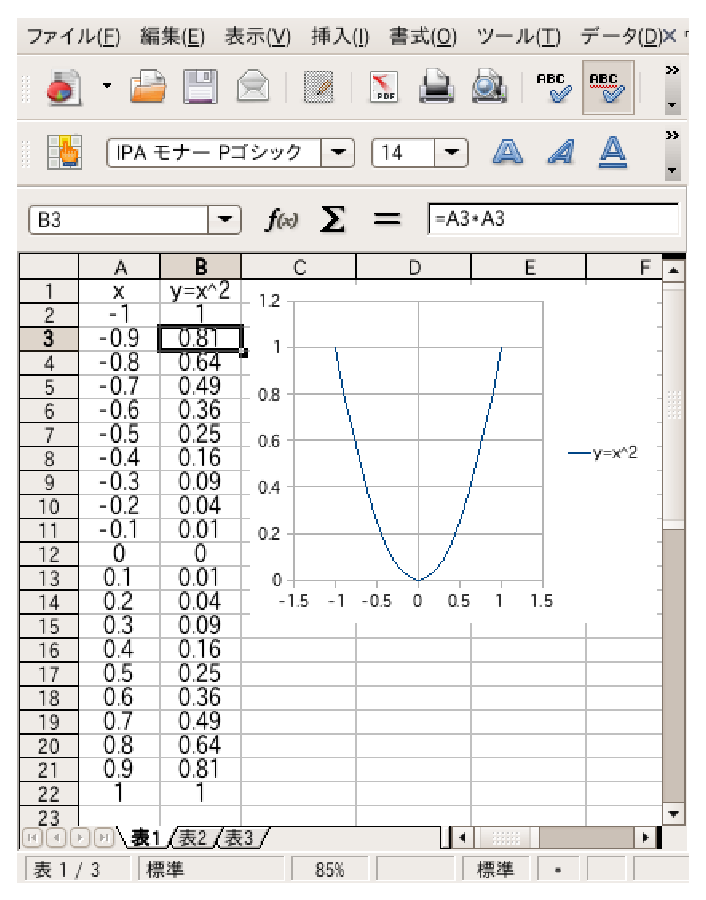
\includegraphics[width=7.3cm]{PC_graph0.eps}
    \caption{$y=x^2$のグラフを描いたところ\label{fig:PC_graph0}}
\end{figure}

\begin{figure}
    \centering
    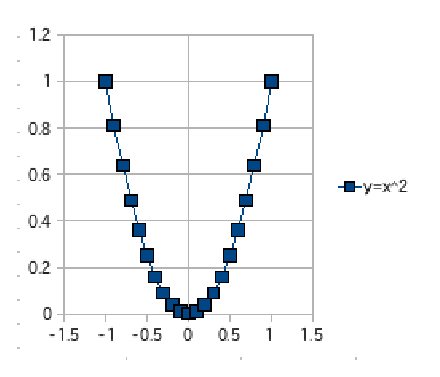
\includegraphics[width=4.5cm]{PC_graph1.eps}
    \caption{グラフ線にマークを入れると見にくい\label{fig:PC_graph1}}
\end{figure}

\begin{faq}{\small\textgt{なぜA1から選ぶのですか? 数値が入っているのは
A2からですよね?} ... それによってセルB1が一緒に選ばれるところがミソです。
そうすることで, B1の内容が, 凡例に表示されるのです。これによって, グラフが
わかりやすくなります。}\end{faq}

\begin{freqmiss}{\small\textgt{関数のグラフを描く時, 横軸の値が不適切な
範囲になる} ... 上の例や下の問で, 「散布図」を選ばずに, 「折れ線」などを選んでしまう
とそうなります。出来上がったグラフをよくチェックしましょう。}\end{freqmiss}

{\small 注: レポートや論文, プレゼン等で使うグラフ(人様に見せるグラフ)をパソコン
で作るときは, 以下に気をつけよう:
\begin{itemize}
\item 複数の関数をひとつのグラフに重ねて描くときは, どの線が
どの関数に対応しているのかを, 必ず凡例などで明記すること。
\item 線の区別をするときは, カラーだけに頼るのではなく, 線の種類
や太さも変えて区別すること(線のどこかをダブルクリックすると, それらを
変更できるウィンドウが出てくる)。これは\textgt{色盲の人への配慮}。
\end{itemize}}

%-----------------------------

{\small 注: 次の問題も含め, 以後, パソコンでグラフを描く問題は, 
レポートではグラフのプリントアウトを掲載せよ。グラフをワープロの
文書にコピー&ペーストすると, レイアウトが楽だし, 複数のグラフを
1枚の紙に印刷するときにも便利。数値データはプリントアウトしなくてもよい。}

\begin{q}\label{q:comp_graph0} パソコンの表計算ソフトを使って, 
次の関数を, $-1 \le x \le 1$の範囲でグラフに描け。重ねて描け。
\begin{edaenumerate}<3>
\item $y=x$
\item $y=x^2$
\item $y=x^3$
\end{edaenumerate}
{\small ヒント: $x$の値は, まとめてひとつの列(A列)にしてよい。B2には「=A2」, C2には「=A2*A2」, D2には「=A2*A2*A2」
と入れて, それぞれ列の下のほう(22行)までコピー・ペースト。B1, C1, D1にそれぞれの関数
の凡例を書き込み(B1には"y=x"とか), A1からD22をマウスで一気に選んでグラフを描けば, 
自動的に3つの線が重なったグラフになる。答えは図\ref{fig:PC_graph2}のようになる。}\end{q}
\begin{figure}
    \centering
    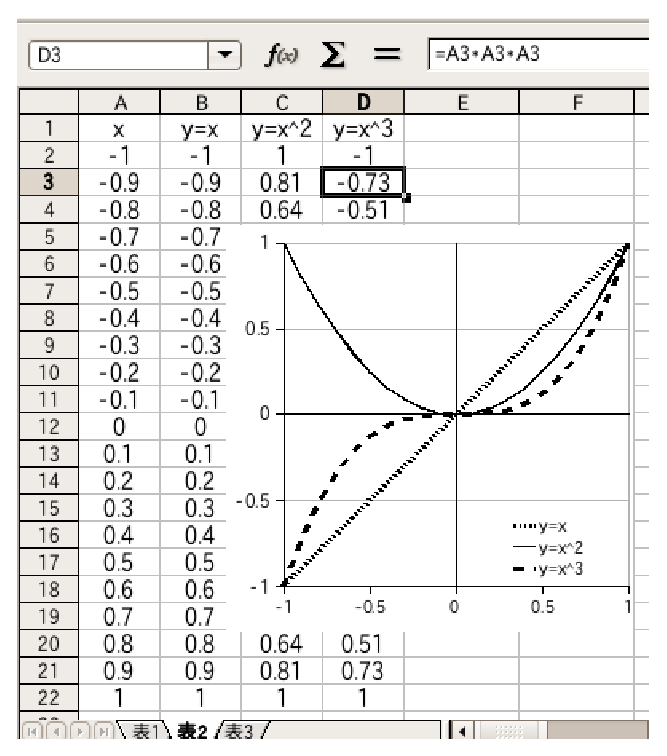
\includegraphics[width=7.0cm]{PC_graph2.eps}
    \caption{$y=x,\, y=x^2,\, y=x^3$のグラフ\label{fig:PC_graph2}}
\end{figure}

\begin{freqmiss}{\small\textgt{複数のグラフを重ねて描くとき, 
どの線が何を表しているかを表示しない} ... そういうレポートは 
減点されるかもしれませんね...}\end{freqmiss}
\hv



\section{関数のグラフと不等式の解}\index{ふとうしき@不等式}

\begin{exmpl}\label{exmpl:ineq001} $x+2<2x-1$という不等式を満たす$x$
はどのような値だろうか? これを式変形すると$3<x$となるから, 
この不等式は$x$が3より大きな値で成立する。\qed\end{exmpl}

\begin{exmpl}\label{exmpl:ineq003} 不等式
\begin{eqnarray}
x^2-x-2<0\label{eq:x2_x_2le0}
\end{eqnarray}
を考える(このように2次式に
関する不等式を2次不等式という)。これを
式変形すると$(x-2)(x+1)<0$である。\eref{eq:th_order_8}
より, $(x-2)$と$(x+1)$は, 片方が負で片方が正のはず。
明らかに$-2<1$だから$x-2<x+1$。小さいほうが負, 大きい方が
正になるはずだから, $x-2<0$かつ$0<x+1$。これを
整理して, $-1<x<2$。これが, この不等式の解。\qed\end{exmpl}

例\ref{exmpl:ineq001}のような単純な不等式は式変形だけで
解けるが, 例\ref{exmpl:ineq003}のような複雑な不等式は, 
ちょっとめんどくさかった。そういうとき, グラフが役立つ。
\eref{eq:x2_x_2le0}の左辺を抜き出して$y=x^2-x-2$という関数
を考えると, そのグラフは図\ref{fig:2Dpoly_graph}の
右端のようになる。\eref{eq:x2_x_2le0}は, この関数を使って$y<0$
と表される。つまり, このグラフが$x$軸よりも下に来るような
ときの$x$の値の範囲を見い出せばよい。明らかにそれは
$-1<x<2$であり, 上の解と一致する。\\

同様に考えれば, 以下の定理が成り立つことがわかるだろう: 
2次方程式$ax^2+bx+c=0$が$x=\alpha$と$x=\beta$という実数解を
持つ時($0<a$, $\alpha<\beta$とする), 不等式
\begin{eqnarray}
ax^2+bx+c<0\label{eq:alg_2ineq_1}
\end{eqnarray}
の解は「$\alpha<x<\beta$」であり, 不等式
\begin{eqnarray}
ax^2+bx+c>0\label{eq:alg_2ineq_2}
\end{eqnarray}
の解は「$x<\alpha$又は$\beta<x$」である。

なぜか? $y=ax^2+bx+c$と
おくと, そのグラフは$x=\alpha$と$x=\beta$で$x$軸と交わり, 
しかも$a>0$なので下に凸の放物線となる。そのグラフが$x$軸
よりも下にある状況や(\eref{eq:alg_2ineq_1}), 上に
ある状況(\eref{eq:alg_2ineq_2})を見い出せばよい。また, 
\eref{eq:alg_2ineq_1}, \eref{eq:alg_2ineq_2}について, 
$<$を$\leq$に置き換えたものについては, その解も
$<$を$\leq$に置き換えたものになることは明らかだろう。

\begin{q}\label{q:alg_ineq1} $x$は実数とする。以下の2次不等式を解け。
\begin{edaenumerate}
\item $x^2+x-6<0$
\item $x^2+5x+6\geq 0$
\item $x^2+3x+1\geq 0$
\end{edaenumerate}
\end{q}

\begin{exmpl} 不等式
\begin{eqnarray}
x^2+x+1>0\label{eq:x2_x_1gt0}
\end{eqnarray}
の解はどうなるだろう?
関数$y=x^2+x+1$のグラフは, 図\ref{fig:2Dpoly_graph}の
左端のようになる。\eref{eq:x2_x_1gt0}は, この関数を使って$y>0$
と表されるから, このグラフが$x$軸よりも上に来るときの
$x$の範囲を言えばよい。といっても, 見るからにこのグラフは
$x$がどんな値でも$x$軸より上にある。従って, 「解は全ての実数」である。\qed\end{exmpl}

\begin{freqmiss}{\small\textgt{↑これを「全ての実数解」という}
 ... なんかおかしくね? 解は何? と聞かれてるんだよ...}\end{freqmiss}

上の例をちょっと変えて, 
\begin{eqnarray}
x^2+x+1<0\label{eq:x2_x_1lt0}
\end{eqnarray}
という不等式の解はどうだろう? そう, 「解なし」だ!

\begin{freqmiss}\label{ex:2dim_ineq_irr}{\small\textgt{
不等\eref{eq:x2_x_1lt0}の解を以下のように間違える:
\begin{eqnarray*}
\frac{-1-\sqrt{3}\,i}{2} < x < \frac{-1+\sqrt{3}\,i}{2}\,\,\,\,\,\, \text{これは間違い!}
\end{eqnarray*}} ... この式には意味がありません。なぜなら, \textgt{虚数には大小関係は存在しない}
からです(例えば, $1+i$とか$5i$はこの「範囲」に入っているかどうか, 言えますか?)。
不等式は普通, 実数の範囲で考えます。}\end{freqmiss}
\mv

\eref{eq:x2_x_1lt0}は, 本来はグラフを使わないで, 以下のように解くべきだ。まず, 
\begin{eqnarray}
\Bigl(x+\frac{1}{2}\Bigr)^2+\frac{3}{4}\label{eq:2dim_ineq_irr5}
\end{eqnarray}
と平方完成する。$(x+\frac{1}{2})^2$は$x$がどんな実数値をとっても0以上だから, 
この式は常に3/4以上。ということは, この式はマイナスになり得ない。従って「解なし」。

このように, 「左辺=0」が実数解を持たないような2次不等式は, 
\eref{eq:2dim_ineq_irr5}のように平方完成して考えねばならない。\hv

\begin{q}\label{q:alg_ineq2}
実数$x$に関する以下の不等式を解け。 
\begin{eqnarray*}
&&(1)\,\,\,\,\,\,\,\,x^2+x+1>0\\
&&(2)\,\,\,\,\,\,\,\,x^2+x+1<0\\
&&(3)\,\,\,\,\,\,\,\,\frac{x+1}{x-1}>0\\
&&(4)\,\,\,\,\,\,\,\,x^2-4x+4<0\\
&&(5)\,\,\,\,\,\,\,\,x^2-4x+4\leq0\\
&&(6)\,\,\,\,\,\,\,\,x^2-4x+4\geq0\\
&&(7)\,\,\,\,\,\,\,\,x^2-4x+4>0
\end{eqnarray*}
{\small ヒント: (3)は分母が0になったら困るから$x\neq1$を前提として, 
両辺に$(x-1)^2$を掛ける。もし, $(x-1)$を両辺にかけてしまうと, 
$x$が1より小さいときに不等号が逆転してしまう(\pref{eq:th_order_3}
の\eref{eq:th_order_3}より)。それを処理するのは面倒。
$(x-1)^2$は0以上だから, 両辺にかけても不等号はかわらない。(4)〜(7)は, 左辺が
$(x-2)^2$であることに注意。}
\end{q}


\section{偶関数・奇関数}
関数$f(x)$が, 恒等的に
\begin{eqnarray}f(-x)=f(x)\end{eqnarray}
を満たすとき, $f(x)$を\underline{偶関数} \index{ぐうかんすう@偶関数}と呼ぶ(定義)。
また, 関数$f(x)$が恒等的に
\begin{eqnarray}f(-x)=-f(x)\label{eq:def_odd_func}\end{eqnarray}
を満たすとき, $f(x)$を\underline{奇関数} \index{きかんすう@奇関数}と呼ぶ(定義)。
偶関数や奇関数は, 他の関数よりも, 何かと扱いが楽である。何か関数を相手に
するときは, まずその関数が偶関数や奇関数か調べよう。もしそうならラッキー!なのだ。\hv

{\small 注: \eref{eq:def_odd_func}を, なぜかわざわざ「$f(x)=-f(-x)$」と変形して
覚える人がいる。間違いではないのだが, この形は, 奇関数の性質を証明する時に
使いづらく, 面倒である。素直に\eref{eq:def_odd_func}の形で覚えよう。}

\begin{q}\label{q:func_evenodd0} 偶関数とは何か? 奇関数とは何か?\end{q}
\mv

既に学んだように, 関数$y=f(x)$のグラフを$y$軸に関して対称移動したら
関数$y=f(-x)$のグラフになる(\ref{sec:func_trans}節の定理5)。ところが
偶関数なら, $f(-x)$はもとの関数$f(x)$に等しい。すなわち, 偶関数のグラフは, 
$y$軸に関して対称移動しても, もとの関数のグラフと一致してしまう。
従って, \textgt{偶関数のグラフは$y$軸に関して対称}である。例えば, 
$y=x^2$は偶関数だが, そのグラフ(図\ref{fig:parab_inverse}左)は
確かに$y$軸に関して対称である。

一方, 関数$y=f(x)$のグラフを原点に関して対称移動したら関数$y=-f(-x)$のグラフに
なる(\ref{sec:func_trans}節の定理6)。ところが, 奇関数なら, 
$-f(-x)$はもとの関数である$f(x)$に等しい。すなわち, 奇関数のグラフは, 
原点に関して対称移動しても, もとの関数のグラフと一致してしまう。
従って, \textgt{奇関数のグラフは原点に関して対称}である。
例えば, $y=ax$ (図\ref{fig:proportion})
や, $y=1/x$や$y=x^3-x$は奇関数だが, それらのグラフ (図\ref{fig:parab_inverse}右, 
図\ref{fig:xxx-x})は確かに原点に関して対称である。

\begin{q}\label{q:func_evenodd1} 以下の各関数$f(x)$について, 偶関数か奇関数か
(もしくはどちらでもないか)を判定し, $y=f(x)$のグラフを描け。
\begin{enumerate}
\item $f(x)=4x^4-5x^2+1$\\ ヒント: $x$軸との交点も考えよ。
\item $f(x)=x+x^2$
\item $f(x)=x-x^3$
\item $f(x)=1/(1+x^2)$\\ ヒント: $x=0$と$x\rightarrow \pm \infty$ではどうなるか? 
\end{enumerate}\end{q}

\begin{faq}{\small\textgt{↑このグラフはパソコンで描くのですか?}
... いえ, 手書きでOK。今後も, 「グラフを描け」は, 「パソコンで」とか「表計算ソフトで」
という指示のある場合はパソコン, それ以外は手書き。}\end{faq}

\begin{freqmiss}{\small\textgt{偶関数の定義を「グラフが$y$軸に関して対称であるような関数」
と言ったり, 奇関数の定義を「グラフが原点に関して対称であるような関数」と言ってしまう}
... それらが定義なら, それらを使って以下の問題を解けますか?}\end{freqmiss}

\begin{q}\label{q:func_evenodd2} 以下を証明せよ:
\begin{enumerate}
\item 偶関数と偶関数の積は偶関数。
\item 奇関数と奇関数の積は偶関数。
\item 偶関数と奇関数の積は奇関数。
\item 偶関数と偶関数の和は偶関数。
\item 奇関数と奇関数の和は奇関数。
\item 偶関数と奇関数の和は, 偶関数でも奇関数でもなくなることがある。(ヒント: 例を挙げればよい。)
\end{enumerate}\end{q}

\begin{q}\label{q:func_evenodd25} 以下の関数について, 偶関数か, 奇関数か, 
いずれでもないか, 判定せよ。
\begin{eqnarray}
f(x)=\Bigl\{(1+x^2+x^4)^3+\frac{1}{x^2+x^4}\Bigr\}^8
\end{eqnarray}\end{q}
↑こんな複雑な関数のグラフなんか, 描ける気がしないだろう。
それでもまだ, 「グラフがなんちゃらに関して対称」とかで偶関数や
奇関数を定義したいなら, なんとかしてグラフを描いてくれ!
\mv

\begin{q}\label{q:func_evenodd28} 関数$f(x)=ax^n$を考える($a$は0以外の任意の実数, $n$は自然数)。$n$が偶数の時は$f(x)$は偶関数であり, $n$が奇数の時は$f(x)$は奇関数であることを証明せよ。\end{q}
\mv

\begin{faq}{\small\textgt{偶関数・奇関数って, 偶数・奇数と関係
ありますか?} ... 言葉が似てるだけに, 前問のように何かしら関係が
あります。また, 問\ref{q:func_evenodd2}で見たことは, 偶数どうしの積が
偶数になるとか, 奇数どうしの積が奇数になるとかに似ています。ただし, 
偶数と奇数の和は奇数だけど, 偶関数と奇関数の和は奇関数とは限りません。
そもそも別の概念だから, どこかが違っているのは当然と言えば当然。}\end{faq}

\begin{faq}{\small\textgt{偶関数の定義を述べよという問題で, 「$f(-x)=f(x)$」と
答えたら不正解になりました。なぜ?}
... 省略しすぎ! せめて「$f(-x)=f(x)$を満たすような関数$f(x)$のこと」
くらいは書かなきゃ, 何のことかわかりません。}\end{faq}
\hv


\section{合成関数}\label{sec:gousei_kansu}
2つの関数$f(x), g(x)$を考える。ある数を$f(x)$に入れると別の数が
返ってくるが, その返ってきた数を次に$g(x)$に入れると, さらに別の
数が返ってくる。このように, 2つの関数$f(x), g(x)$を段階的に続けて
使うことで, 新たな関数ができる。それを「$f(x)$と$g(x)$の
合成関数」\index{ごうせいかんすう@合成関数}といい, $g(f(x))$と書く。
例を見てみよう:

\begin{exmpl} 以下の2つの関数の合成関数を考えよう:
\begin{eqnarray*}
f(x)=x+1,\quad\quad g(x)=x^2
\end{eqnarray*}
例えば$x=1$について, $f(1)=1+1=2$, $g(2)=2^2=4$となる。従って, $g(f(1))=4$である。

合成関数は, 2段めの関数の独立変数$x$に1段めの関数を代入したものである。この場合は, 
\begin{eqnarray}g(f(x))=g(x+1)=(x+1)^2\label{eq:gousei_kansu6}\end{eqnarray}
となる。これに$x=1$を代入すると, 確かに4になる。

\eref{eq:gousei_kansu6}は次のように考えてもよい:
\begin{eqnarray}g(f(x))=\{f(x)\}^2=(x+1)^2\end{eqnarray}
結果は同じである。

合成の順序を変えると, 違った合成関数になることに注意しよう。上の例では, 
\begin{eqnarray}f(g(x))=f(x^2)=x^2+1\label{eq:gousei_kansu7}\end{eqnarray}
である。\eref{eq:gousei_kansu6}と\eref{eq:gousei_kansu7}は明らかに違う関数だ!
(例おわり)\end{exmpl}\mv

$g(f(x))$と書かれるとき, 内側に1段めの関数が, 外側に2段めの関数が
書かれることに注意しよう。左から見ていくと2段めが先に来て1段めが後に来るので, 
順序が混乱する人がいるが, 「何を何に代入するか」と考えれば
自然に納得できるだろう。

\begin{q}\label{q:gouseikansu0} 2つの関数$f(x)=\sqrt{x}$, $g(x)=1+x^2$について, 
$g(f(x))$と$f(g(x))$をそれぞれ求めよ。
\end{q}
\hv


\section{逆関数}\label{sec_gyakukansu}

一般に, 関数$y=f(x)$の$x$と$y$を入れ替えてできる関数$y=g(x)$を, 
関数$f(x)$の\underline{逆関数} \index{ぎゃくかんすう@逆関数}と呼ぶ(定義)。

\begin{exmpl}\label{exmpl:func_inv1} 関数$y=2x$は, $x$と$y$を入れ替えると
$x=2y$となる。これを$y$について解けば$y=x/2$となる。従って, 
$y=2x$の逆関数は$y=x/2$である。(例おわり)\end{exmpl}

\begin{q}\label{q:func_inv0} 以下の関数の逆関数をそれぞれ求めよ。ただし, $a$, $b$は任意の定数とする。
\begin{edaenumerate}
\item $y=2x+1$
\item $y=1/(x-1)$
\item $y=a/x$
\item $y=-x+b$
\end{edaenumerate}
\end{q}\mv

逆関数はどういうイメージのものだろうか? 一般に, 
関数$y=f(x)$を, 数$x$から数$y$への「変換装置」みたいな
ものと考えれば, $x$は「入り口」, $y$は「出口」だ。
従って, $x$と$y$を入れ替えるということは, この装置の
働きを逆行させ, 「出口から入って入り口から出る」ということ。
つまり, $y=f(x)$で変換された数を, 変換前の数に戻す
のが逆関数$y=g(x)$だ。

そう考えると, $g(x)$が$f(x)$の逆関数なら, 逆の立場も言える, つまり
$f(x)$は$g(x)$の逆関数である, ということがわかるだろう。

\begin{exmpl}\label{exmpl:func_inv2} 関数$y=2x$に$x=3$という数を入れると, 
$y=6$という数に変換される。この数を改めて$x$として関数$y=x/2$ (これが$y=2x$の
逆関数であることは例\ref{exmpl:func_inv1}でみたとおり) に入れると, 
$y=6/2=3$となる。確かに最初の$x$の値に戻った。(例おわり)\end{exmpl}\mv

さて, 逆関数にはひとつ面白い性質がある: 
\textgt{$f(x)$と$g(x)$が互いに逆関数であるとき, 恒等的に
\begin{eqnarray}g(f(x))=f(g(x))=x\label{eq:generaleq}\end{eqnarray}
となる}のだ。なぜだろう? 
$f(x)$は, $x$を別の数に移す関数だが, 逆関数$g(x)$はそれを
もとの数$x$に戻す関数だ。だから, $g(f(x))$は, $x$をいったん別の数に移しても
それを元に戻すので, 結局は何もしないに等しい。つまり, $g(f(x))$は$x$をそのまま$x$に
しておく関数である。つまり, 恒等的に$g(f(x))=x$が成り立つ。
同様に, $f(g(x))=x$も恒等的に成り立つ。\qed

\begin{exmpl}\label{exmpl:func_inv3} 例\ref{exmpl:func_inv1}でみた
ように, 関数$y=2x$の逆関数は$y=x/2$である。前者を$f(x)$, 後者を$g(x)$と
してみよう。つまり$f(x)=2x$, $g(x)=x/2$とする。
\begin{eqnarray}
&&f(g(x))=2g(x)=2\times\frac{x}{2}=x\\
&&g(f(x))=\frac{f(x)}{2}=\frac{2x}{2}=x
\end{eqnarray}
確かに\eref{eq:generaleq}が成り立ってる! (例おわり)\end{exmpl}

\begin{q}\label{q:func_inv1} $0\le x$とする。$f(x)=x^2$, $g(x)=\sqrt{x}$について,
 \eref{eq:generaleq}が成り立つことを確かめよ。($x^2$と$\sqrt{x}$は互いに逆関数である。)\end{q}\mv

$f(x)$と$g(x)$が互いに逆関数であるとき, $y=g(x)$は$x=f(y)$と同じことだから, $y=f(x)$のグラフにおいて
$x$軸と$y$軸を取り換えたものが$x=f(y)$, つまり$y=g(x)$のグラフになる
(図\ref{fig:func_revfunc})。

\begin{figure}[h]
    \centering
    \includegraphics[width=6cm]{func_revfunc.eps}
    \caption{関数$y=f(x)$とその逆関数$y=g(x)$のグラフは$y=x$に関して互いに対称である。\label{fig:func_revfunc}}
\end{figure}

グラフ上で$x$軸と$y$軸を取り換えるときに, 直線$y=x$
だけは不変である。直線$y=x$は$x$軸と$y$軸のちょうど
中間の, 折り返しの位置にあるからだ。あたかも直線$y=x$に
沿って鏡があるように$y=f(x)$のグラフを反転したものが
$x=f(y)$, すなわち$y=g(x)$のグラフになる。従って, 
\textgt{逆関数のグラフはもとの関数のグラフを直線$y=x$に関して対称移動したものだ。}
(だからと言って, これを逆関数の定義としてはいけない。)

\begin{q}\label{q:func_inv2} $y=x^2$と$y=\sqrt{x}$を重ねてグラフに描け.\end{q}

\begin{freqmiss}{\small\textgt{$y=\sqrt{x}$のグラフを, 原点で$y$軸に
突き刺さる角度で描いてしまう} ... $y=x^2$のグラフは放物線なので原点で$x$軸
に接しますよね。$y=\sqrt{x}$はその逆関数なのだから, $y$軸にやさしく接する
はず。突き刺さってはダメ!}\end{freqmiss}

%上で見たように, 逆関数のグラフは$y=x$に関して対称移動したグラフになるので, 
%もともと$y=x$に関して対称なグラフを持つ関数は, 自分自身が自分自身の逆関数になる。\\
\mv

たまに逆関数と逆数を混同する人がいるが, 全く別の概念だ。
たとえば, 例\ref{exmpl:func_inv1}で見たように, $y=2x$の逆関数は$y=x/2$だが, 
$2x$の逆数は$1/(2x)$だ。また, 問\ref{q:func_inv0}で見たように, 
逆関数が自分自身になる関数は多いが, 逆数が自分自身になる数は1と$-1$しかない。\\

\begin{q}\label{q:func_inv3} 次の関数のグラフを, パソコンを使って, \\
$0 \le x \le 1$の範囲で重ねて描け。レポートには, そのグラフのプリントアウトを貼り付けること。
\begin{edaenumerate}<3>
\item $y=x$
\item $y=x^2$
\item $y=x^3$
\item $y=x^4$
\item $y=x^{1/2}$
\item $y=x^{1/3}$
\item $y=x^{1/4}$
\end{edaenumerate}
ヒント: 表計算ソフトでべき乗をするときは\^ \,という記号を使う。
例えばセルA3の3乗は「=A3$\hat{\,\,\,}$3」とする。セルA3の$1/3$乗
は, 「=A3$\hat{\,\,\,}$(1/3)」とする(括弧を忘れないこと!)。
(6), (7)は, 刻みを細かくしよう。
\end{q}

この問でわかるように, $n$を自然数とすると, $y=x^n$のグラフと$y=x^{1/n}$のグラフは, 
直線$y=x$に関して対称である。それらは互いに逆関数だからだ。

また, この形の関数を, 一般に$y=x^\alpha$とおくと, そのグラフは, $\alpha$
によって形が系統的に変わる。この$\alpha$のような数, すなわち
独立変数$x$や従属変数$y$ではなくて関数の性質を決定するような
数のことを, \underline{パラメータ}\index{パラメータ}
% (parameter)
と呼ぶ
\footnote{「パラメータ」と言う言葉には「媒介変数」という別の意味もあるが, それはいずれ説明する。}。
例えば\eref{eq:y_ax_plus_b0}の$a$と$b$もパラメータである。「パラメータが変わるとどうなるか」
という目で関数を理解しよう。そうすると, 「この現象はこういう関数で表現できるのでは?」
という勘が働くようになる。\mv

\begin{faq}{\small\textgt{パソコンでグラフ描くのめんどくさいです。テキストに
載ってるグラフを見るだけでよいのでは?}
... それはダメ。「見るだけ」では心に残らないよ。「見ればわかる」
ことでも, 自分で手を動かしてやってみないと, 心に残らないのです。
人間はそういうもの。このテキストは, パソコンの計算やグラフ描画を通じて
実感・納得するよう設計しています。そのかわり, 他の本にあるような
細かい証明や理屈は載せていません。そうやって学習者の負担を軽くし, 
そのぶん, 生物資源学類で出てくる実例を増やしたり, より高度で
有用な数学を盛り込んでいます。}\end{faq}


\section{陰関数}\index{いんかんすう@陰関数}

今から学ぶのは, ちょっと変わった関数である。いや, 正確には「関数」とは
言えない, 「関数もどき」である。

$y=f(x)$という関数では, $x$の値を代入すれば$y$の値が決まる。しかし, 
ふたつの変数$x, y$を対応づけるのは, このように$y=$の形になっている
関数だけではない。$x^2+xy+y^2-1=0$のように, $x$と$y$が混在する
ような2変数関数が0に等しい, という式でも, いちおう$x$と$y$は対応する。このように, $x$と$y$の
2変数関数$F(x, y)$について, $F(x, y)=0$という方程式で$x$と$y$が対応する場合, この対応関係を
\underline{陰関数} (implicit function)と呼ぶ(定義)。

代表例として, 以下のような陰関数がある。

\begin{q}\label{q:func_circle0} $r$を正の実数の定数とする。陰関数
\begin{eqnarray}
x^2+y^2-r^2=0\label{eq:func_circle0}
\end{eqnarray}
のグラフは(ただし$r>0$とする), 原点を中心とする半径$r$の円になることを示せ。\end{q}
\mv

陰関数を式変形すれば$y=f(x)$の形に整理できることもあるが, 
多くの場合は難しい。ひとつの$x$の値に, 複数の$y$の値が対応する
こともあるからだ。例えば, \eref{eq:func_circle0}は, 
\begin{eqnarray}
y=\pm\sqrt{r^2-x^2}\label{eq:func_circle00}
\end{eqnarray}
と変形できるが, 右辺の$\pm$が嫌らしい。例えば$x=0$に対して
$y=r$と$y=-r$という2つの数が対応してしまう。そもそも関数とは, 
ひとつの$x$に対してひとつの$y$を対応付けるものだ(後に学ぶ「写像」
という概念)。従って, 陰関数は, 厳密な意味では関数ではないのだ。\hv

陰関数にも, グラフの対称性や平行移動, 拡大といった考え方が適用できる。

\begin{exmpl}\label{ex:func_imp0} ある陰関数$F(x,y)=0$の
グラフを$x$軸の正方向に$a$, $y$軸の正方向に$b$だけ平行移動
すると, $F(x-a, y-b)=0$のグラフになる。なぜか?

陰関数$F(x,y)=0$のグラフ上の任意の点Pを考える。その座標を$(x_0, y_0)$とする。
すなわち, $F(x_0, y_0)=0$である。
点Pを$x$軸の正方向に$a$, $y$軸の正方向に$b$だけ平行移動した先の点
を点P$_1$とし, その座標を$(x_1, y_1)$とする。当然, $x_1=x_0+a$
かつ$y_1=y_0+b$である。従って$x_0=x_1-a$
かつ$y_0=y_1-b$である。これを$F(x_0, y_0)=0$に代入すると, 
$F(x_1-a, y_1-b)=0$である。従って, 点P$_1$は陰関数$F(x-a, y-b)=0$
のグラフ上にある。(例おわり)\end{exmpl}

\begin{comment}
一般に, 陰関数$F(x, y)=0$のグラフに関して, 以下の定理が成り立つ
(例\ref{ex:func_imp0}では, 定理1を示した):\\
定理1) $x$軸の正方向に$a$, $y$軸の正方向に$b$だけ平行移動すると, $F(x-a, y-b)=0$のグラフになる。\\
定理2) $x$軸方向に$a$倍, $y$軸方向に$b$倍だけ拡大すると, $F(x/a, y/b)=0$のグラフになる。\\
定理3) $x$軸に関して対称移動すると, $F(x, -y)=0$のグラフになる。\\
定理4) $y$軸に関して対称移動すると, $F(-x, y)=0$のグラフになる。\\
定理5) 原点に関して対称移動すると, $F(-x, -y)=0$のグラフになる。\\
定理6) 恒等的に$F(x, -y)=F(x, y)$なら, $x$軸に関して対称。\\
定理7) 恒等的に$F(-x, y)=F(x, y)$なら, $y$軸に関して対称。\\
定理8) 恒等的に$F(-x, -y)=F(x, y)$なら, 原点に関して対称。\hv

定理2$\sim$定理5の証明は, 形式的には例\ref{ex:func_imp0}で
示した定理1の証明とほぼ同じ。以下にポイントだけを示す:

定理2) $x_1=ax_0$, $y_1=by_0$とする。

定理3) $x_1=x_0$, $y_1=-y_0$とする。

定理4) $x_1=-x_0$, $y_1=y_0$とする。

定理5) $x_1=-x_0$, $y_1=-y_0$とする。

定理6の証明: $F(x, -y)=0$のグラフは, $F(x, y)=0$のグラフを
$x$軸に関して対称移動したもの。ところが, 恒等的に$F(x, -y)=F(x, y)$
なのだから, それは$F(x, y)=0$のグラフに一致するはず。つまり
このグラフは$x$軸に関して対称移動しても元のグラフに一致する。
従って, $x$軸に関して対称である。\qed

定理7, 定理8の証明は, 定理6の証明とほぼ同様。\mv
\end{comment}

\begin{q}\label{q:func_imp1} ($x$, $y$)平面上で, 点$(3, -1)$を中心とする, 半径2の円
を表す陰関数を求めよ。
%\begin{enumerate}
%\item 原点を中心とし, $x$軸方向に径$a$の長軸を持ち, $y$軸方向に径$b$の短軸を
%持つような楕円。ただし$a, b$は正の定数とし, $a>b$とする。
%\end{enumerate}
\end{q}

%\begin{q}\label{q:func_imp2} 以下を示せ。
%\begin{enumerate}
%\item $x^2y^2-1=0$のグラフは, $x$軸に関して対称, 
%$y$軸に関しても対称, 原点に関しても対称。
%\item $x^2+xy+y^2-3=0$のグラフは, 原点に関して対称だが, 
%$x$軸に関して対称ではなく, $y$軸に関しても対称ではない。
%\end{enumerate}
%\end{q}
%問\ref{q:func_imp2}のような陰関数のグラフは, ぱっと思い描くのは難しい。しかし, 
%上で示した定理を使えば, グラフを描く前に, その対称性がわかってしまうのだ。
%数学の論理の素晴らしさはそのようなところにある。
%\hv

\begin{comment}
\begin{exmpl}\label{exmp:func_imp3} $x^2-y^2=1$のグラフを描いてみよう。

まず, このグラフが$x$軸や$y$軸と交わる点を求めよう(なぜなら, $x=0$や$y=0$を
代入するのは簡単だから!)。

$x=0$のときは, $-y^2=1$, つまり$y^2=-1$となり, $y$は実数解を持たない。つまり, 
グラフは$x=0$では点を持たない, すなわち, このグラフは$y$軸を横切ったり$y$軸
に接したりすることはない。

次に, $y=0$のときは, $x^2=1$, つまり$x=\pm1$である。つまりこのグラフは, 
$(1, 0)$, $(-1, 0)$を通る(これが$x$軸との交点)。

次に, グラフの対称性を調べよう。$x^2-y^2-1=0$と変形し, $F(x, y)=x^2-y^2-1$
とすると, この陰関数は, $F(x, y)=0$と書ける。簡単な暗算で, $F(-x, y)=F(x, y)$と
$F(x, -y)=F(x, y)$が成り立つことがわかる。従って, このグラフは$x$軸と$y$軸の
それぞれに関して対称である(上の定理6と定理7)。

次に, $x$や$y$がどんどん大きくなるとこのグラフはどうなるか, 調べよう。
$x$や$y$が1000や10000のように大きな数になると, $F(x, y)=x^2-y^2-1=0$で示される
$x$と$y$の関係の中では, 定数項である「$-1$」は, 相対的に無視できる
(100万円や1億円を持っている人は, 1円にはこだわらない!)。
従って,  この陰関数は, $x^2-y^2\fallingdotseq0$となる。因数分解すると, 
$(x-y)(x+y)\fallingdotseq0$すなわち, $x-y\fallingdotseq0$または$x+y\fallingdotseq0$
となる。つまり, 直線$y=x$または直線$y=-x$に次第に近づく。これらが漸近線である。

これだけの手がかりで, ほとんどグラフは描けるが, 心配な人のために, もうひと押ししよう。
この陰関数は, $y^2=x^2-1$, すなわち$y=\pm\sqrt{x^2-1}$と変形できる。
$0<x, 0<y$の範囲(つまりグラフの第一象限\footnote{$0<x,\, 0<y$の領域。
$x$軸と$y$軸で区切られる平面の右上部分のこと。})に限定すると, $y=\sqrt{x^2-1}$
であり, この関数は$x$に関して単調に増加する。従って, $x$が大きくなるに従って, 
点$(1, 0)$から, 漸近線$y=x$に向けて単調に近づく線を描くはずだ。それを対称性
によって$y$軸の左側や$x$軸の下側にコピーする。結果として, 
図\ref{xx_minus_yy_eq_1}のようなグラフになる\footnote{実は, 図\ref{xx_minus_yy_eq_1}は, 
\pref{fig:parab_inverse}の図\ref{fig:parab_inverse}右で見たような双曲線を回転させたものになっている。正確に言うと, 
$y=1/(2x)$で表される双曲線を, 90度, 右回りに回転させたのが図\ref{xx_minus_yy_eq_1}である。}。
なお, なぜか図\ref{fig:hyperbola_NG}のように漸近線から離れて行くグラフを描いてしまう人がいるので注意!
\begin{figure}
    \centering
      \includegraphics[width=5cm]{xx_minus_yy_eq_1.eps}
      \caption{$x^2-y^2=1$のグラフ。点線は漸近線($y=\pm x$)。\label{xx_minus_yy_eq_1}} 
\end{figure}
(例おわり)\end{exmpl}
\hv

\begin{q}\label{q:func_imp4} 以下の関数について, それぞれグラフを描け。漸近線がある場合は
漸近線を点線で描き込み, その方程式も述べよ。:
\begin{edaenumerate}
\item $x^2-y^2=-1$
\item $4x^2-y^2=1$
\item $x^2-y^2=9$
\item $x^2+y^2/4=1$
\end{edaenumerate}\end{q}

\begin{figure}
    \centering
      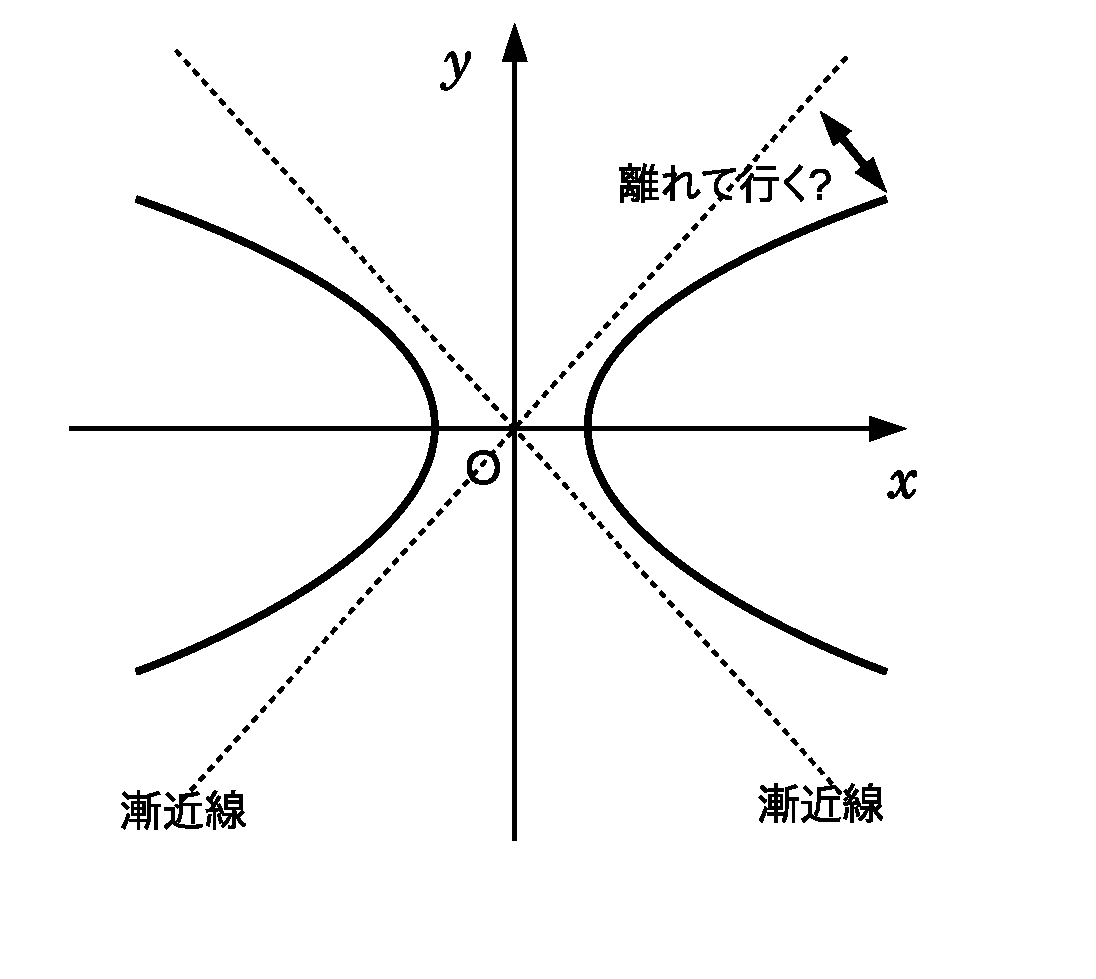
\includegraphics[width=5cm]{hyperbola_NG.eps}
      \caption{よくある\textgt{\large{ダメな}}グラフ。漸近線は
グラフが近づいて行く線なので, 離れて行くのは間違い!\label{fig:hyperbola_NG}} 
\end{figure}
\hv
\end{comment}

\section{関数のグラフを描く手順}
ここで, 関数のグラフを手で描く手順をまとめておこう:
\begin{itemize}
\item $x$の全範囲で関数はつながっているかチェック。$1/x$のように割り算が入った関数は, 「0での割り算」の
ところで関数が途切れる。陰関数は, $x$のとりうる範囲がかなり限定されることもある
(例えば$x^2+y^2=1$は$-1\le x \le 1$でしか定義されない)。
\item $x=0$での$y$の値($y$軸との共有点)を調べる。無いとき(虚数解になるとき)はグラフは$y$軸を通らない。
\item $y=0$での$x$の値($x$軸との共有点)を調べる。無いとき(虚数解になるとき)はグラフは$x$軸を通らない。
\item 関数の対称性を調べる($x$を$-x$にしてみたり$y$を$-y$にしてみたり)。
\item よく知っている関数の平行移動や拡大, 縮小, 対称移動, 和などにならないか調べる。
\item $x$や$y$が$\infty$や$-\infty$に行くときの様子を調べる。
%\item 漸近線があるかどうか, 調べる。
\item それでもよくわからないときは, $x$に適当な数(なるべく計算しやすい値)
をいくつか代入して$y$の値を求め, グラフにプロットしてみる。
\end{itemize}

\begin{faq}{\small\textgt{高校で数IIIを習ったときは, 関数を微分して増減表を
作って, それをもとに関数のグラフを描きました。それじゃダメですか?}
... もちろんいいですよ。でも, ここで学んだ, 「微分を使わないやり方」も有用です。
複雑な関数, 特に陰関数は, 微分したりそれが0になる$x$を求めたりが大変だったり
するからね。それに, 漸近線は増減表からは出ないよね。ここでやったように, 関数の
おおまかな性質を検討するだけでも, いろんな関数のグラフを, 漸近線を
含めてうまく描けます。そういう大局的な見方は, いろんな関数をイメージする
ための強力な武器です。実際, 複雑な関数のグラフはパソコンで描け
ばいいのですが, それを正しく行い, 結果を吟味するには, 
ここで学んだ考え方が有用なのです。}\end{faq}
\hv


\section*{演習問題}

\begin{exq}\label{q:Michaelis_Menten} 次式は, 酵素が介在する
化学反応の速度を説明する, ミカエリス・メンテンの式というものである: 
\begin{eqnarray}
v=\frac{V_{\text{max}}[S]}{K_{\text{m}}+[S]}\label{eq:Michaelis_Menten0}
\end{eqnarray}
$V_{\text{max}}$と$K_{\text{m}}$は正の定数。
$v$は化学反応の速度(単位時間あたり, 単位体積あたりに生成される
化学物質の量), $[S]$は基質(化学反応の材料となる物質)の濃度である。
この式は, $v$を$[S]$の関数として表している。
\begin{enumerate}
\item $[S]=0$のとき$v=0$であることを示せ。
\item $[S]\rightarrow\infty$の極限で, $v$は$V_{\text{max}}$に限りなく近づいていくことを示せ。
\item $[S]=K_{\text{m}}$のとき, $v=V_{\text{max}}/2$となることを示せ。
\item 以上を参考にして, \eref{eq:Michaelis_Menten0}のグラフを描け。
横軸を$[S]$, 縦軸を$v$とせよ。基質の濃度は0以上なので, $0\leq[S]$としてよい。
\item $y=1/v$, $x=1/[S]$として, \eref{eq:Michaelis_Menten0}を$y$と$x$の関係式(一次式)に変形せよ。
それをグラフに描いた時, 切片と傾きにはどのような意味があるか?
\end{enumerate}\end{exq}\mv

{\small 参考(酵素化学が専門の橋本義輝先生のコメント): 学生はミカエリスメンテン式を, $V_{\text{max}}$と$K_{\text{m}}$
が決まってるので任意の$[S]$の時の$v$がわかる式と理解しているようです。しかし, 酵素学では, $V_{\text{max}}$と$K_{\text{m}}$にそれぞれ意味があるので、実験的に求めた複数の$[S]$と$v$の関係からミカエリスメンテン式を使って$V_{\text{max}}$と$K_{\text{m}}$を求めることになります(表裏一体で、どちらから眺めるかの違いですが...)。}

%\begin{exq}\label{q:func_1_1_x2} 以下の関数のグラフを描け。漸近線がある場合は
%漸近線を点線で描き込み, その方程式も述べよ。
%\begin{eqnarray}
%y=\frac{1}{1-x^2}
%\end{eqnarray}
%ヒント: 分母が0になるような$x$では, グラフは発散して途切れる。
%よくわからない, という人は, $x$に$0, 0.1, 0.5, 0.9, 1.1, 2, 3$などの
%値を代入してみよ。
%\end{exq}

\begin{exq}\label{q:func_evenodd_gousei} $K_1(x), K_2(x)$を奇関数, 
$G_1(x), G_2(x)$を偶関数とする。以下の関数を, 奇関数か, 偶関数か, 
どちらとも言えないか, 示せ(根拠も述べよ)。
\begin{edaenumerate}
\item $K_1(K_2(x))$
\item $G_1(G_2(x))$
\item $K_1(G_1(x))$
\item $G_1(K_1(x))$
\item $K_1(x)$の逆関数
\item $G_1(x)$の逆関数
\end{edaenumerate} 
\end{exq}\mv

%\begin{exq}\label{q:func_even_and_odd} 奇関数であり, なおかつ偶関数
%でもあるような関数はあるか? あるなら, どのような関数か? 
%根拠も述べよ。ヒント: 陰関数は関数ではないので除外して考える。\end{exq}

\begin{exq}\label{q:func_imp_th2} 陰関数$F(x, y)=0$のグラフに関して, 
\begin{enumerate}
\item $x$軸に関して対称移動すると, $F(x, -y)=0$のグラフになることを示せ。
\item 恒等的に$F(x, -y)=F(x, y)$なら, $x$軸に関して対称であることを示せ。
\item $x$軸方向に$a$倍, $y$軸方向に$b$倍だけ拡大すると, $F(x/a, y/b)=0$のグラフになることを示せ。
\item 以上を参考にして, 以下の2つの陰関数のグラフをそれぞれ描け:\\
(1)  $x^2-y^2=1$   (2)  $(x^2/4)+(y^2/9)=1$
\end{enumerate}
\end{exq}\mv

%\begin{exq}\label{q:func_inverse_invariant} (発展)
%\begin{enumerate}
%\item 一般に, 関数$f(x)$のグラフが直線$y=x$に関して対称であれば, その
%関数の逆関数は自分自身であることを証明せよ。
%\item 問\ref{q:func_inv0}の関数以外で, 逆関数が自分自身になるような
%関数の例を3つ挙げよ(定数や係数の値だけが異なるものは認めない)。
%% F(x, y)=F(y, x)となる陰関数でF(x, y)=0としたものをyについて解けばよい。
%\end{enumerate}
%\end{exq}

%\begin{exq}\label{q:function_English} 以下の言葉を英訳せよ:
%\begin{edaenumerate}
%\item 関数
%\item 極限
%\item 独立変数
%\item パラメータ
%\end{edaenumerate}
%\end{exq}\mv
\hv



\section*{問題の解答}

%\noindent{\textbf{答}}\ref{q:func_trans0}  略(実際に各点を$xy$平面にプロットしてみよ)。\mv

\noindent{\textbf{答}}\ref{q:func_trans1}  $y=f(x)$の
グラフ上の任意の点Pを考える。その座標を$(x_0, y_0)$とする。
$y_0=f(x_0)$が成り立つ。

定理2の証明: 点Pを$x$軸方向に$a$倍して移動した先の点,
すなわち$(ax_0, y_0)$を, あらためて点P$_2$とし, 
その座標を$(x_2, y_2)$と置く。すなわち, 
$x_2=ax_0,\, y_2=y_0$である。すなわち, $x_0=x_2/a, y_0=y_2$
である。これを$y_0=f(x_0)$に代入すると, $y_2=f(x_2/a)$となる。
従って, 点P$_2$は$y=f(x/a)$のグラフの上にある。\qed

%定理3$\sim$定理6の証明は, 定理2の証明と形式的には
%ほぼ同じである。以下にポイントだけを示す(君はちゃんとやること!)。

%定理3では, 移動先の点$(x_0, ay_0)$を点P$_3$とし, 
%その座標を$(x_3, y_3)$とする。

定理4の証明: 点Pを$x$軸に関して対称移動した先の点, 
すなわち$(x_0, -y_0)$を, あらためて点P$_4$とし, 
その座標を$(x_4, y_4)$と置く。すなわち, 
$x_4=x_0,\, y_4=-y_0$である。すなわち, $x_0=x_4, y_0=-y_4$
である。これを$y_0=f(x_0)$に代入すると, $-y_4=f(x_4)$, 
すなわち$y_4=-f(x_4)$となる。従って, 点P$_4$は
$y=-f(x)$のグラフの上にある。\qed
\mv

\noindent{\textbf{答}}\ref{q:func_trans2}  
\begin{enumerate}
\item $y=(x-1)^{2}+2$
\vspace{0.1cm}
\item $y=3(x/2)^2=3x^2/4$
\vspace{0.1cm}
\item $y=x^2$を(図\ref{fig:x2_trans}左上), まず$x$軸方向に2倍することで, 
\begin{eqnarray}y=\Bigr(\frac{x}{2}\Bigl)^2\end{eqnarray}
になる(図\ref{fig:x2_trans}中上)。さらに$x$軸方向に1移動することで, 
\begin{eqnarray}y=\Bigr(\frac{x-1}{2}\Bigl)^2\end{eqnarray}
になる(図\ref{fig:x2_trans}右上)。
\item $y=x^2$を(図\ref{fig:x2_trans}左下), まず$x$軸方向に1移動することで, 
\begin{eqnarray}y=(x-1)^2\end{eqnarray}
になる(図\ref{fig:x2_trans}中下)。さらに$x$軸方向に2倍することで, 
\begin{eqnarray}y=\Bigr(\frac{x}{2}-1\Bigl)^2\end{eqnarray}
になる(図\ref{fig:x2_trans}右下)。
\end{enumerate}
\begin{figure}[h]
    \centering
      \includegraphics[width=7.0cm]{x2_trans.eps}
      \caption{$y=x^2$の2段階の変形。順序が違えば結果も違う。点線は$y=x^2$。\label{fig:x2_trans}}
\end{figure}


\noindent{\textbf{答}}\ref{q:func_trans3}  図\ref{2x_plus_1_etc}参照。
\begin{enumerate}
\item $y=2x$のグラフを上に($y$軸方向に)1移動。
\item $y=(x+1)^2+2$だから, $y=x^2$のグラフを左($x$軸の負の方向)に1, 上に2移動。
\item $y=1/x$のグラフを上($y$軸の正の方向)に2移動。
\item $y=2-2/(x+1)$だから, $y=1/x$のグラフを縦に2倍し, 上下反転し, 左($x$軸の負の方向)に1, 上に2移動。
$x=0$のときに$y=0$となるので, 原点を通る。
\end{enumerate}

\begin{figure}[h]
    \centering
      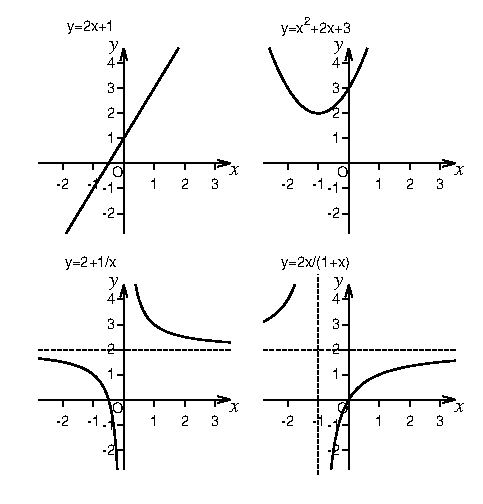
\includegraphics[width=6cm]{2x_plus_1_etc.eps}
      \caption{問\ref{q:func_trans3}のこたえ。点線は漸近線。\label{2x_plus_1_etc}}
\end{figure}
\mv

\noindent{\textbf{答}}\ref{q:func_line0} 
\begin{enumerate}
\item $y=3x-2$
\item \eref{eq:lineeq}より, $y=2(x+1)+1$, \\すなわち$y=2x+3$。
\item \eref{eq:lineeq2p}より, 
\begin{eqnarray}y=\frac{-3-1}{4-2}(x-2)+1\end{eqnarray}
すなわち$y=-2x+5$。
\end{enumerate}
\mv

\noindent{\textbf{答}}\ref{q:Fahrenheit} 
\begin{enumerate}
\item $(32, 0)$と$(212, 100)$を通る一次関数(直線の式)を求めればよい。
\begin{eqnarray*}
&&y-0=\frac{100-0}{212-32}(x-32)\quad\text{すなわち, }\\
&&y=\frac{5}{9}(x-32)=\frac{5}{9}\,x-\frac{160}{9}
\end{eqnarray*}
\item
\begin{eqnarray*}
x=\frac{9}{5}\,y+32
\end{eqnarray*}
\item 以下略
\end{enumerate}
\mv
%\noindent{\textbf{答}}\ref{q:x_plus_1_over_x} 略。\mv

%\noindent{\textbf{答}}\ref{q:read_a_graph} 略。\mv

%\noindent{\textbf{答}}\ref{q:read_a_graph_line} 略。\mv

% パソコンの表計算ソフトを使って, 次の関数を, $-1 \le x \le 1$の範囲でグラフにかけ
%\noindent{\textbf{答}}\ref{q:comp_graph0}  略。

% 不等式
%\noindent{\textbf{答}}\ref{q:alg_ineq0} まず$a<b\text{かつ}(x-a)(x-b)<0$とする。\eref{eq:th_order_8}より, $(x-a)$と$(x-b)$の片方は負, もう片方は正。
%ところが, $a<b$より, $-b<-a$。両辺に$x$を足すと, $x-b<x-a$。従って, $x-b$が負で, $x-a$が正である。つまり$x-b<0$かつ$0<x-a$。前者から$x<b$, 後者から$a<x$。この両方が成り立つはずだから, $a<x<b$ (\eref{eq:alg_2ineq_1}の証明おわり)。\\
%次に, $a<b\text{かつ}(x-a)(x-b)>0$とする。\eref{eq:th_order_7}より, $(x-a)$と$(x-b)$は同符号。ともに正のときは, $0<x-a$かつ$0<x-b$。すなわち$a<x$かつ$b<x$。ところが, $a<b$より, $b<x$であれば$a<x$は自動的に成り立つ。従って, $b<x$を満たすだけでよい。一方, ともに負のときは, $x-a<0$かつ$x-b<0$。すなわち$x<a$かつ$x<b$。ところが, $a<b$より, $x<a$であれば自動的に$x<b$が成り立つ。従って, $x<a$を満たすだけでよい。以上から, $x<a$または$b<x$
%(\eref{eq:alg_2ineq_2}の証明おわり)。\qed

\noindent{\textbf{答}}\ref{q:alg_ineq1} 
\begin{enumerate}
\item 左辺=0の解は$x=-3, 2$。$\therefore\,-3<x<2$
\item 左辺=0の解は$x=-3, -2$。$\therefore\,x \leq -3,\, -2 \leq x$
\item 左辺=0の解は$x=\frac{-3\pm\sqrt{5}}{2}$。よって, 
\begin{eqnarray*}
x \leq \frac{-3-\sqrt{5}}{2},\,\,\, \frac{-3+\sqrt{5}}{2} \leq x
\end{eqnarray*}
\end{enumerate}

\noindent{\textbf{答}}\ref{q:alg_ineq2} 
\begin{enumerate}
\item 左辺=$(x+1/2)^2+3/4$。これは$x$がどんな実数値でも正の値をとる。従って, この不等式は, すべての実数値$x$について成り立つ。
\item 前問と同様に考えれば, この不等式はどんな実数値にも成り立たない(解を持たない)。
\item (略解) $x<-1,\, 1<x$
\item (略解) 解なし。
\item (略解) $x=2$
\item (略解) 全ての実数。
\item (略解) 2以外の全ての実数。
\end{enumerate}
\mv

\noindent{\textbf{答}}\ref{q:func_evenodd0} 略。「グラフがなんとかに関して対称」とか
書いてしまった人は, もっと真剣に本文を読もう!
\mv

\noindent{\textbf{答}}\ref{q:func_evenodd1}  グラフは図\ref{xxxx_minus_etc}参照。
\begin{enumerate}
\item 偶関数。$y=(x+1)(2x+1)(2x-1)(x-1)$なので, $x$軸との交点は$x=-1, -1/2, 1/2, 1$。
$x\rightarrow \pm \infty$で, $y\rightarrow \infty$。
\item どちらでもない。$y=(1+x)x$なので, $x$軸との交点は$x=-1, 0$。$y=(x+1/2)^2-1/4$なので, 
$y=x^2$のグラフを左に$1/2$, 下に$1/4$移動。
\item 奇関数。$y=-(x+1)x(x-1)$なので, $x$軸との交点は$x=-1, 0, 1$。
$x\rightarrow \infty$で, $y\rightarrow -\infty$。
$x\rightarrow -\infty$で, $y\rightarrow \infty$。
(本文の例\ref{exmpl:func_xxx_x}の, $y=x^3-x$のグラフ, つまり図\ref{fig:xxx-x}を, 上下反転したものとも言える。)
\item 偶関数。$x\rightarrow \pm \infty$で, $y\rightarrow 0$。つまり$x$軸に漸近する。
$x=0$のとき$y=1$。ピークを尖らせたらダメ!
\end{enumerate}
\mv

\begin{figure}[h]
    \centering
      \includegraphics[width=8.5cm]{xxxx_minus_etc.eps}
      \caption{問\ref{q:func_evenodd1}のこたえ。\label{xxxx_minus_etc}}
\end{figure}

\noindent{\textbf{答}}\ref{q:func_evenodd2}  $f_1(x),\, f_2(x)$を任意の偶関数, 
$g_1(x),\, g_2(x)$を任意の奇関数とする。定義より, 
\begin{eqnarray*}
&&f_1(-x)=f_1(x),\quad f_2(-x)=f_2(x)\\
&&g_1(-x)=-g_1(x),\quad g_2(-x)=-g_2(x)
\end{eqnarray*}
である。さて, 
\begin{enumerate}
\item $F(x)=f_1(x)f_2(x)$とすると, 
\begin{eqnarray*}
F(-x)=f_1(-x)f_2(-x)=f_1(x)f_2(x)=F(x)
\end{eqnarray*}
従って, $F(x)$は偶関数。\qed
\vspace{0.1cm}
\item $F(x)=g_1(x)g_2(x)$とすると, 
\begin{eqnarray*}
F(-x)&=&g_1(-x)g_2(-x)=\{-g_1(x)\}\{-g_2(x)\}\\
     &=&g_1(x)g_2(x)=F(x)
\end{eqnarray*}
従って, $F(x)$は偶関数。\qed
\vspace{0.1cm}
\item $F(x)=f_1(x)g_1(x)$とすると, 
\begin{eqnarray*}
F(-x)&=&f_1(-x)g_1(-x)=f_1(x)\{-g_1(x)\}\\
     &=&-f_1(x)g_1(x)=-F(x)
\end{eqnarray*}
従って, $F(x)$は奇関数。\qed
\vspace{0.1cm}
\item $F(x)=f_1(x)+f_2(x)$とすると, 
\begin{eqnarray*}
F(-x)=f_1(-x)+f_2(-x)=f_1(x)+f_2(x)=F(x)
\end{eqnarray*}
従って, $F(x)$は偶関数。\qed
\vspace{0.1cm}
\item $F(x)=g_1(x)+g_2(x)$とすると, 
\begin{eqnarray*}
F(-x)&=&g_1(-x)+g_2(-x)=-g_1(x)-g_2(x)\\
     &=&-\{g_1(x)+g_2(x)\}=-F(x)
\end{eqnarray*}
従って, $F(x)$は奇関数。\qed
\vspace{0.1cm}
\item 例えば偶関数$y=1$と奇関数$y=x$の和: $y=1+x$は, 偶関数でも奇関数でもない。\qed
\end{enumerate}
\mv

\noindent{\textbf{答}}\ref{q:func_evenodd25} 略解: $f(-x)=f(x)$となることは
暗算でも確認できる。答は偶関数。注: $f(-x)=f(x)$を満たせば偶関数なのだから(それが定義), 
それを確認すれば十分である。グラフなど描く必要はない。\mv

\noindent{\textbf{答}}\ref{q:gouseikansu0}
$g(f(x))=1+x$ (ただし$x\ge0$), $f(g(x))=\sqrt{1+x^2}$\mv

\noindent{\textbf{答}}\ref{q:func_inv0} 
\begin{enumerate}
\item $x$と$y$を入れ替えると$x=2y+1$。変形すると, $y=(x-1)/2$。
\item $x$と$y$を入れ替えると$x=1/(y-1)$。変形すると, $y=1+1/x$。
\item $x$と$y$を入れ替えると$x=a/y$。変形すると, $y=a/x$。
\item $x$と$y$を入れ替えると$x=-y+b$。変形すると, $y=-x+b$。
\end{enumerate}
注: (3), (4)では逆関数が自分自身になっていることに注意せよ。\mv

\noindent{\textbf{答}}\ref{q:func_inv1} $g(f(x))=\sqrt{f(x)}=\sqrt{x^2}=|x|$。$x$は0以上だから, これは$x$に恒等的に等しい。また, 
$f(g(x))=(g(x))^2=(\sqrt{x})^2=x$。
\mv

\noindent{\textbf{答}}\ref{q:func_inv2} 図\ref{xx_and_sqrt_x}参照。
\mv

\noindent{\textbf{答}}\ref{q:func_inv3} 図\ref{x_or_xx_etc}参照。
\mv

\begin{figure}[h]
    \centering
      \includegraphics[width=7cm]{xx_and_sqrt_x.eps}
      \caption{問\ref{q:func_inv2}の答。図中, "sqrt(x)"とあるのは$\sqrt{x}$のこと。
直線$y=x$に関して対称であることに注意。どの線も点$(1, 1)$を通る。\label{xx_and_sqrt_x}}
\end{figure}

\begin{figure}[h]
    \centering
      \includegraphics[width=7cm]{x_or_xx_etc.eps}
      \caption{問\ref{q:func_inv3}の答。$y=x$の上側にあるのが, $x^{1/2},\, x^{1/3},\, x^{1/4}$。
どの線も点$(1, 1)$を通る。\label{x_or_xx_etc}}
\end{figure}

\noindent{\textbf{答}}\ref{q:func_circle0} 三平方の定理より$x^{2} + y^{2}$は, 原点から点$(x,\,y)$までの距離の二乗。与式より, 
これが$r^2$に常に等しいので, 原点から各点までの距離は常に$r$である。原点から一定距離$r$
にある点の集合は, 原点を中心とする半径$r$の円である。\qed
\mv

\noindent{\textbf{答}}\ref{q:func_imp1} 
原点中心, 半径$2$の円を表す陰関数は, \eref{eq:func_circle0}で$r=2$として, 
$x^2+y^2-4=0$。これを$x$方向に3, $y$方向に$-1$だけ移動すると(例\ref{ex:func_imp0}より), \\
$(x-3)^2+(y+1)^2-4=0$。\mv
%\item 原点中心, 半径$1$の円を表す陰関数は, $x^2+y^2-1=0$。これを$x$軸方向に$a$倍, 
%$y$軸方向に$b$倍だけ伸ばすと(定理2より), 
%\begin{eqnarray}\frac{x^2}{a^2}+\frac{y^2}{b^2}-1=0\end{eqnarray}
%\end{enumerate}

\begin{comment}
\noindent{\textbf{答}}\ref{q:func_imp2}
\begin{enumerate}
\item $F(x, y)=x^2y^2-1$とする。任意の$x, y$について, 
$F(-x, y)=F(x, -y)=F(-x, -y)=F(x, y)$が恒等的に成り立つので, 
定理5, 6, 7より, $F(x, y)=0$のグラフは$x$軸と$y$軸と原点に
関して対称。\qed
\item $F(x, y)=x^2+xy+y^2-3$とする。任意の$x, y$について, 
$F(-x, -y)=F(x, y)$が恒等的に成り立つので原点対称。しかし, 
点$(1, 1)$は$F(x, y)=0$を満たすが, その点を$x$軸と$y$軸に
関してそれぞれ対称に移動した点$(-1, 1)$と$(1, -1)$は, $F(x, y)=0$
を満たさないので, このグラフ上には存在しない(反例)。従って, この
グラフは$x$軸に関しても$y$軸に関しても対称ではない。\qed
\end{enumerate}
\hv

\noindent{\textbf{答}}\ref{q:func_imp4} 図\ref{4xx_minus_yy_eq_1_etc}参照。
(1)では, $y=\pm\sqrt{x^2+1}$となるが, $x$が十分に大きいと根号の中の1は
$x^2$よりずっと小さいので無視でき, $y\fallingdotseq\pm\sqrt{x^2}=\pm x$と
なる。従って, $y=x$と$y=-x$が漸近線。(2)では, $y=\pm\sqrt{4x^2-1}$となるが, 
$x$が十分大きい時は, $y\fallingdotseq\pm\sqrt{4x^2}=\pm2x$となる。従って, 
$y=2x$と$y=-2x$が漸近線。(3)では, $y=\pm\sqrt{x^2-9}$となるが, 
$x$が十分大きい時は, $y\fallingdotseq\pm\sqrt{x^2}=\pm x$となる。従って, 
$y=x$と$y=-x$が漸近線。(4)では漸近線は存在しない(なぜなら, $x$が大きな数に
なると$y$は虚数になるし, $y$が大きな数になると$x$は虚数になる。虚数の点は
グラフには現れない)。

\begin{figure}
    \centering
    \includegraphics[width=7cm]{4xx_minus_yy_eq_1_etc.eps}
    \caption{問\ref{q:func_imp4}のこたえ。それぞれ, 点線は漸近線。}\label{4xx_minus_yy_eq_1_etc}
\end{figure}
\vv
\end{comment}



